\documentclass[11pt]{article}

\usepackage[T1]{fontenc}
\usepackage[utf8]{inputenc}
\usepackage{lmodern}
\usepackage{microtype}
\usepackage[margin=0.82in]{geometry}
\usepackage{amsmath,amssymb,mathtools}
\usepackage{booktabs}
\usepackage{array}
\usepackage{enumitem}
\usepackage[most]{tcolorbox}
\usepackage{tikz}
\usetikzlibrary{arrows.meta,calc,decorations.pathreplacing,positioning,patterns}
\usepackage{fancyhdr}
\usepackage{hyperref}
\usepackage{needspace}
\usepackage{graphicx}
\usepackage{multicol}

\hypersetup{
  colorlinks=true,
  linkcolor=blue!55!black,
  urlcolor=blue!55!black,
  pdftitle={Exercise 10.3: Max Version of Hilbert's Inequality},
  pdfauthor={OpenAI}
}

\setlength{\parindent}{0pt}
\setlength{\parskip}{0.62em}
\setlist[itemize]{leftmargin=1.55em,itemsep=0.25em,topsep=0.25em}
\setlist[enumerate]{leftmargin=1.75em,itemsep=0.35em,topsep=0.3em}
\allowdisplaybreaks
\setcounter{tocdepth}{1}

\pagestyle{fancy}
\fancyhf{}
\lhead{Exercise 10.3 Tutorial}
\rhead{Max Hilbert Inequality}
\cfoot{\thepage}
\setlength{\headheight}{14pt}

\definecolor{navy}{RGB}{24,55,93}
\definecolor{softblue}{RGB}{235,244,252}
\definecolor{softgreen}{RGB}{236,248,239}
\definecolor{softyellow}{RGB}{255,249,226}
\definecolor{softred}{RGB}{253,239,239}
\definecolor{softgray}{RGB}{245,246,248}
\definecolor{softpurple}{RGB}{245,239,251}

\newtcolorbox{problemBox}{
  enhanced,
  colback=softblue,
  colframe=navy,
  boxrule=0.8pt,
  arc=2mm,
  title=The problem,
  fonttitle=\bfseries,
  breakable
}

\newtcolorbox{ideaBox}[1][Key idea]{
  enhanced,
  colback=softgreen,
  colframe=green!45!black,
  boxrule=0.7pt,
  arc=2mm,
  title={#1},
  fonttitle=\bfseries,
  breakable
}

\newtcolorbox{warningBox}[1][Watch out]{
  enhanced,
  colback=softyellow,
  colframe=orange!65!black,
  boxrule=0.7pt,
  arc=2mm,
  title={#1},
  fonttitle=\bfseries,
  breakable
}

\newtcolorbox{solutionBox}[1][Solution step]{
  enhanced,
  colback=white,
  colframe=navy!75,
  boxrule=0.8pt,
  arc=2mm,
  title={#1},
  fonttitle=\bfseries,
  breakable
}

\newtcolorbox{definitionBox}[1][Definition]{
  enhanced,
  colback=softgray,
  colframe=black!45,
  boxrule=0.6pt,
  arc=2mm,
  title={#1},
  fonttitle=\bfseries,
  breakable
}

\newtcolorbox{extraBox}[1][Extra insight]{
  enhanced,
  colback=softpurple,
  colframe=purple!55!black,
  boxrule=0.7pt,
  arc=2mm,
  title={#1},
  fonttitle=\bfseries,
  breakable
}

\newcommand{\N}{\mathbb{N}}
\newcommand{\norm}[1]{\left\lVert #1\right\rVert}
\newcommand{\abs}[1]{\left|#1\right|}
\newcommand{\Kmn}{K_{m n}}
\newcommand{\HN}{H_N}

\begin{document}

\begin{center}
  {\LARGE\bfseries Exercise 10.3: Max Version of Hilbert's Inequality}\\[0.35em]
  {\Large A square-root weight, Cauchy--Schwarz, and a sharp constant}\\[0.7em]
  {\large A step-by-step tutorial for a high-school reader}
\end{center}

\vspace{0.4em}

\begin{ideaBox}[What you will learn]
By the end of this tutorial, you will be able to:
\begin{itemize}
  \item read the double sum as a weighted matrix expression;
  \item see why the line \(m=n\) divides the problem into two simple regions;
  \item prove two useful estimates involving square roots;
  \item use a carefully chosen weight \(w_n=1/\sqrt n\) inside Cauchy--Schwarz;
  \item prove the constant \(4\) is the smallest possible universal constant.
\end{itemize}
\end{ideaBox}

\tableofcontents
\newpage

\section{The exercise, stated carefully}

\begin{problemBox}
Let \(a=(a_1,a_2,\ldots)\) and \(b=(b_1,b_2,\ldots)\) be real sequences whose squares have finite sums:
\[
  \sum_{m=1}^{\infty}a_m^2<\infty,
  \qquad
  \sum_{n=1}^{\infty}b_n^2<\infty.
\]
Show that
\[
 \boxed{\displaystyle
 \abs{\sum_{m=1}^{\infty}\sum_{n=1}^{\infty}
       \frac{a_m b_n}{\max\{m,n\}}}
 <4
 \left(\sum_{m=1}^{\infty}a_m^2\right)^{1/2}
 \left(\sum_{n=1}^{\infty}b_n^2\right)^{1/2}}
 \tag{1}
\]
when both sequences are nonzero. Then prove that no constant smaller than \(4\) can work for every pair of sequences.
\end{problemBox}

The displayed exercise does not put absolute-value signs around the double sum. We will prove the stronger estimate (1). Since every real number \(S\) satisfies \(S\leq |S|\), the requested inequality follows immediately.

\begin{warningBox}[A small point about the strict inequality]
If one sequence is identically zero, then both sides are zero, so the literal statement \(0<0\) is false. The fully precise version is
\[
 \abs{S(a,b)}\leq 4\norm{a}_2\norm{b}_2
\]
for all square-summable sequences, with strict inequality when both \(a\) and \(b\) are nonzero. This is the version proved below.
\end{warningBox}

\subsection{The infinite-vector length}

For a finite vector, Pythagoras gives the length
\[
  \sqrt{a_1^2+a_2^2+\cdots+a_N^2}.
\]
For an infinite sequence, we use the same idea:
\[
  \norm{a}_2
  :=\left(\sum_{m=1}^{\infty}a_m^2\right)^{1/2}.
\]
A sequence with \(\norm{a}_2<\infty\) is called \emph{square-summable}, or an \(\ell^2\) sequence.

\subsection{The kernel matrix}

Set
\[
  K_{mn}:=\frac{1}{\max\{m,n\}}.
\]
Then the double sum is
\[
  S(a,b)=\sum_{m=1}^{\infty}\sum_{n=1}^{\infty}K_{mn}a_m b_n.
\]
The beginning of the matrix \((K_{mn})\) is
\[
\begin{pmatrix}
1 & \frac12 & \frac13 & \frac14 & \frac15 & \cdots\\[2pt]
\frac12 & \frac12 & \frac13 & \frac14 & \frac15 & \cdots\\[2pt]
\frac13 & \frac13 & \frac13 & \frac14 & \frac15 & \cdots\\[2pt]
\frac14 & \frac14 & \frac14 & \frac14 & \frac15 & \cdots\\[2pt]
\frac15 & \frac15 & \frac15 & \frac15 & \frac15 & \cdots\\[2pt]
\vdots & \vdots & \vdots & \vdots & \vdots & \ddots
\end{pmatrix}.
\]
Notice that the matrix is symmetric: \(K_{mn}=K_{nm}\).

\section{The geometry hidden inside \(\max\{m,n\}\)}

The line \(m=n\) divides the grid of pairs \((m,n)\) into two regions:
\[
  K_{mn}
  =\frac{1}{\max\{m,n\}}
  =\begin{cases}
      \dfrac1m,&m\geq n,\\[5pt]
      \dfrac1n,&n>m.
    \end{cases}
  \tag{2}
\]

\begin{center}
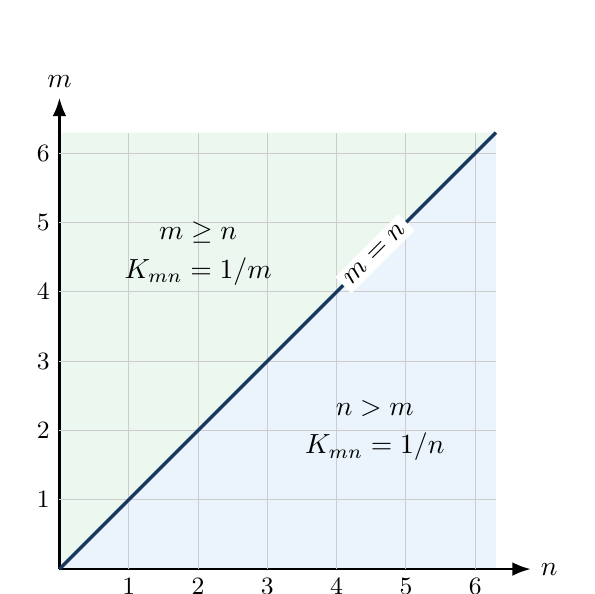
\begin{tikzpicture}[scale=0.88,>=Latex]
  \fill[softblue] (0,0) -- (6.3,0) -- (6.3,6.3) -- cycle;
  \fill[softgreen] (0,0) -- (0,6.3) -- (6.3,6.3) -- cycle;
  \draw[->,thick] (0,0) -- (6.8,0) node[right] {$n$};
  \draw[->,thick] (0,0) -- (0,6.8) node[above] {$m$};
  \foreach \x in {1,...,6}{
    \draw[black!20] (\x,0)--(\x,6.3);
    \draw[black!20] (0,\x)--(6.3,\x);
    \node[below,font=\small] at (\x,0) {\x};
    \node[left,font=\small] at (0,\x) {\x};
  }
  \draw[very thick,navy] (0,0)--(6.3,6.3);
  \node[rotate=45,fill=white,inner sep=2pt] at (4.55,4.55) {$m=n$};
  \node[align=center] at (2.0,4.55) {$m\ge n$\\[2pt]$K_{mn}=1/m$};
  \node[align=center] at (4.55,2.0) {$n>m$\\[2pt]$K_{mn}=1/n$};
\end{tikzpicture}

\small Figure 1. The maximum becomes simple on each side of the diagonal.
\end{center}

This split is the first major idea. For a fixed row number \(m\), the terms with \(n\leq m\) behave differently from the terms with \(n>m\).

\section{Three tools we need}

\subsection{Cauchy--Schwarz}

For finite lists of real numbers,
\[
  \abs{\sum_j x_jy_j}
  \leq
  \left(\sum_jx_j^2\right)^{1/2}
  \left(\sum_jy_j^2\right)^{1/2}.
  \tag{3}
\]
The same formula works for convergent infinite sums. It also works when the index \(j\) is replaced by a pair \((m,n)\): simply imagine writing all grid points in one long list.

\begin{ideaBox}[Why ordinary Cauchy--Schwarz is not enough]
A first attempt might be to separate \(a_mb_n\) from the kernel \(K_{mn}\). That leads to the sum
\(
\sum_{m,n}K_{mn}^2,
\)
which diverges. The successful proof puts a square-root weight into Cauchy--Schwarz so that each row becomes manageable.
\end{ideaBox}

\subsection{A telescoping sum}

A sum is called \emph{telescoping} when most terms cancel. For example,
\[
\begin{aligned}
 &(\sqrt1-\sqrt0)+(\sqrt2-\sqrt1)+\cdots+(\sqrt m-\sqrt{m-1})\\
 &\hspace{4cm}=\sqrt m.
\end{aligned}
\]
We will compare our sums with expressions of this form.

\subsection{Two square-root estimates}

\begin{solutionBox}[Estimate A: the first part of a row]
For every integer \(m\geq1\),
\[
  \boxed{\displaystyle
  \sum_{n=1}^{m}\frac1{\sqrt n}<2\sqrt m.}
  \tag{4}
\]
Indeed,
\[
  2(\sqrt n-\sqrt{n-1})
  =\frac{2}{\sqrt n+\sqrt{n-1}}
  >\frac1{\sqrt n},
\]
because \(\sqrt n+\sqrt{n-1}<2\sqrt n\). Summing from \(n=1\) to \(n=m\) makes the right-hand comparison telescope:
\[
  \sum_{n=1}^{m}\frac1{\sqrt n}
  <2\sum_{n=1}^{m}(\sqrt n-\sqrt{n-1})
  =2\sqrt m.
\]
\end{solutionBox}

\begin{solutionBox}[Estimate B: the tail of a row]
For every integer \(m\geq1\),
\[
  \boxed{\displaystyle
  \sum_{n=m+1}^{\infty}\frac1{n^{3/2}}<\frac2{\sqrt m}.}
  \tag{5}
\]
For \(n\geq2\),
\[
\begin{aligned}
  2\left(\frac1{\sqrt{n-1}}-\frac1{\sqrt n}\right)
  &=\frac{2}{\sqrt{n-1}\sqrt n(\sqrt n+\sqrt{n-1})}\\
  &>\frac1{n^{3/2}}.
\end{aligned}
\]
The last inequality follows because each \(\sqrt{n-1}\) is smaller than \(\sqrt n\), so the denominator on the first line is smaller than \(2n^{3/2}\). Therefore, for any \(M>m\),
\[
\begin{aligned}
 \sum_{n=m+1}^{M}\frac1{n^{3/2}}
 &<2\sum_{n=m+1}^{M}
 \left(\frac1{\sqrt{n-1}}-\frac1{\sqrt n}\right)\\
 &=2\left(\frac1{\sqrt m}-\frac1{\sqrt M}\right)
 <\frac2{\sqrt m}.
\end{aligned}
\]
Letting \(M\) grow gives (5).
\end{solutionBox}

\section{The decisive weight and the number \(4\)}

Choose the positive weight
\[
  \boxed{w_n=\frac1{\sqrt n}.}
  \tag{6}
\]
For a fixed row \(m\), define its weighted row sum by
\[
  R_m:=\sum_{n=1}^{\infty}K_{mn}w_n.
\]
Using the split (2),
\[
\begin{aligned}
 R_m
 &=\sum_{n=1}^{m}\frac1m\frac1{\sqrt n}
   +\sum_{n=m+1}^{\infty}\frac1n\frac1{\sqrt n}\\
 &=\frac1m\sum_{n=1}^{m}\frac1{\sqrt n}
   +\sum_{n=m+1}^{\infty}\frac1{n^{3/2}}.
\end{aligned}
\tag{7}
\]
Apply (4) and (5):
\[
\begin{aligned}
 R_m
 &<\frac1m(2\sqrt m)+\frac2{\sqrt m}\\
 &=\frac4{\sqrt m}=4w_m.
\end{aligned}
\]
Thus we have proved the central estimate
\[
  \boxed{R_m<4w_m\qquad(m=1,2,\ldots).}
  \tag{8}
\]

\begin{center}
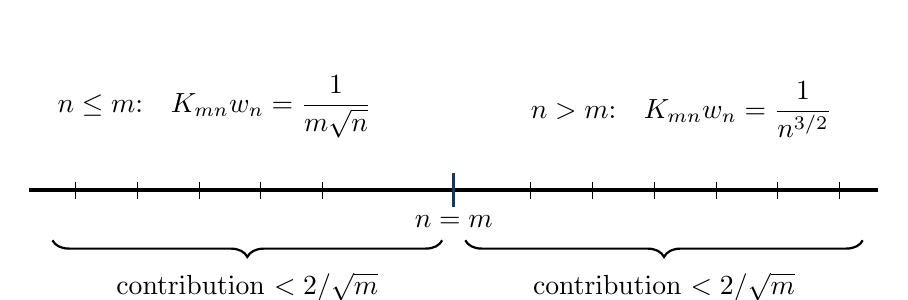
\begin{tikzpicture}[>=Latex,scale=0.98]
  \draw[very thick] (0,0)--(11,0);
  \foreach \x in {0.6,1.4,2.2,3.0,3.8}{\draw (\x,-0.11)--(\x,0.11);}
  \foreach \x in {6.5,7.3,8.1,8.9,9.7,10.5}{\draw (\x,-0.11)--(\x,0.11);}
  \draw[very thick,navy] (5.5,-0.22)--(5.5,0.22);
  \node[below] at (5.5,-0.2) {$n=m$};
  \node[above,align=center] at (2.4,0.55)
    {$n\leq m$:\quad $K_{mn}w_n=\dfrac1{m\sqrt n}$};
  \node[above,align=center] at (8.45,0.55)
    {$n>m$:\quad $K_{mn}w_n=\dfrac1{n^{3/2}}$};
  \draw[decorate,decoration={brace,amplitude=6pt,mirror},thick]
    (0.3,-0.65)--(5.35,-0.65)
    node[midway,below=8pt,align=center] {contribution $<2/\sqrt m$};
  \draw[decorate,decoration={brace,amplitude=6pt,mirror},thick]
    (5.65,-0.65)--(10.8,-0.65)
    node[midway,below=8pt,align=center] {contribution $<2/\sqrt m$};
\end{tikzpicture}

\small Figure 2. The constant \(4\) appears as \(2+2\), one contribution from each side of \(n=m\).
\end{center}

\begin{extraBox}[Where did the square-root weight come from?]
The weight \(n^{-1/2}\) is the natural balance point. Roughly speaking, the left part of (7) and the right part both have size \(m^{-1/2}\). Neither side dominates the other. Later, the sharpness example uses exactly the same shape \(1/\sqrt n\), which is strong evidence that this is the correct choice.
\end{extraBox}

\section{Proof of the inequality}

We now combine the weighted row estimate with Cauchy--Schwarz.

\begin{solutionBox}[Step 1: remove signs]
Because \(K_{mn}>0\),
\[
\begin{aligned}
 \abs{S(a,b)}
 &=\abs{\sum_{m,n\geq1}K_{mn}a_mb_n}\\
 &\leq \sum_{m,n\geq1}K_{mn}|a_m||b_n|.
\end{aligned}
\]
Call the last sum \(T\). Proving \(T<4\norm a_2\norm b_2\) is enough.
\end{solutionBox}

\begin{solutionBox}[Step 2: insert a factor equal to \(1\)]
For every pair \((m,n)\),
\[
 \sqrt{\frac{w_n}{w_m}}
 \sqrt{\frac{w_m}{w_n}}=1.
\]
Therefore,
\[
\begin{aligned}
 K_{mn}|a_m||b_n|
 &=\left(\sqrt{K_{mn}}|a_m|\sqrt{\frac{w_n}{w_m}}\right)
   \left(\sqrt{K_{mn}}|b_n|\sqrt{\frac{w_m}{w_n}}\right).
\end{aligned}
\]
This strange-looking insertion is designed so that the row sum \(R_m\) will appear after squaring.
\end{solutionBox}

\begin{solutionBox}[Step 3: apply Cauchy--Schwarz over all pairs \((m,n)\)]
Equation (3) gives
\[
\begin{aligned}
 T
 &\leq
 \left(\sum_{m,n\geq1}
 K_{mn}a_m^2\frac{w_n}{w_m}\right)^{1/2}
 \left(\sum_{m,n\geq1}
 K_{mn}b_n^2\frac{w_m}{w_n}\right)^{1/2}.
\end{aligned}
\tag{9}
\]
We simplify the first factor by grouping terms with the same \(m\):
\[
\begin{aligned}
 \sum_{m,n\geq1}K_{mn}a_m^2\frac{w_n}{w_m}
 &=\sum_{m=1}^{\infty}\frac{a_m^2}{w_m}
   \sum_{n=1}^{\infty}K_{mn}w_n\\
 &=\sum_{m=1}^{\infty}\frac{a_m^2}{w_m}R_m\\
 &<4\sum_{m=1}^{\infty}a_m^2.
\end{aligned}
\tag{10}
\]
The last line uses \(R_m<4w_m\). Because the kernel is symmetric, exactly the same argument gives
\[
 \sum_{m,n\geq1}K_{mn}b_n^2\frac{w_m}{w_n}
 <4\sum_{n=1}^{\infty}b_n^2.
 \tag{11}
\]
Substitute (10) and (11) into (9):
\[
\begin{aligned}
 T
 &<\left(4\sum_{m=1}^{\infty}a_m^2\right)^{1/2}
    \left(4\sum_{n=1}^{\infty}b_n^2\right)^{1/2}\\
 &=4\norm a_2\norm b_2.
\end{aligned}
\]
Hence
\[
 \boxed{\displaystyle
 \abs{\sum_{m=1}^{\infty}\sum_{n=1}^{\infty}
 \frac{a_m b_n}{\max\{m,n\}}}
 <4\norm a_2\norm b_2.}
\]
\end{solutionBox}

\subsection{Why the infinite double sum is legitimate}

The two squared sums on the right side of (9) are finite by (10) and (11). Cauchy--Schwarz therefore shows that
\[
  \sum_{m,n\geq1}K_{mn}|a_m||b_n|<\infty.
\]
So the original double series converges absolutely. One may also apply the argument first to a finite \(N\times N\) square and then let \(N\to\infty\).

\section{What does it mean for \(4\) to be best possible?}

Suppose somebody claims that a smaller number, such as \(3.99\), works for every pair of sequences. To disprove the claim, we do not need equality at \(4\). We only need examples whose ratio
\[
  \frac{\displaystyle
  \sum_{m,n\geq1}\frac{a_mb_n}{\max\{m,n\}}}
  {\norm a_2\norm b_2}
\]
gets as close to \(4\) as we wish.

\begin{definitionBox}[Sharp or best constant]
The constant \(4\) is \emph{sharp} if the inequality is true with \(4\), but false with every constant \(C<4\).
\end{definitionBox}

The weight used in the proof suggests the right test sequence. The infinite sequence \(1/\sqrt n\) itself is not square-summable, so we cut it off after \(N\) terms.

\section{The near-equality sequences}

For each positive integer \(N\), define
\[
  c_n^{(N)}=
  \begin{cases}
    \dfrac1{\sqrt n},&1\leq n\leq N,\\[5pt]
    0,&n>N.
  \end{cases}
  \tag{12}
\]
Use the same sequence on both sides: \(a=b=c^{(N)}\).

\subsection{Their lengths}

Let
\[
  H_N:=1+\frac12+\frac13+\cdots+\frac1N
\]
be the \(N\)-th harmonic number. Then
\[
  \norm{c^{(N)}}_2^2
  =\sum_{n=1}^{N}\left(\frac1{\sqrt n}\right)^2
  =H_N.
\]
Therefore,
\[
  \norm{a}_2\norm{b}_2=H_N.
  \tag{13}
\]

\subsection{The double sum for these sequences}

Write
\[
  Q_N:=\sum_{m=1}^{N}\sum_{n=1}^{N}
  \frac{1}{\sqrt m\sqrt n\max\{m,n\}}.
\]
The summand is symmetric in \(m,n\). We may double the lower triangle \(n\leq m\), but then the diagonal has been counted twice, so we subtract it once:
\[
\begin{aligned}
 Q_N
 &=2\sum_{m=1}^{N}\sum_{n=1}^{m}
 \frac{1}{m^{3/2}\sqrt n}
 -\sum_{m=1}^{N}\frac1{m^2}\\
 &=2\sum_{m=1}^{N}\frac1{m^{3/2}}
 \left(\sum_{n=1}^{m}\frac1{\sqrt n}\right)
 -\sum_{m=1}^{N}\frac1{m^2}.
\end{aligned}
\tag{14}
\]

\begin{warningBox}[Why subtract the diagonal?]
Doubling one triangular half counts every off-diagonal pair exactly once in each direction, which is correct. But it counts \((m,m)\) twice, while the original square contains it only once. The term on the diagonal is \(1/m^2\).
\end{warningBox}

\section{Show that the ratio approaches \(4\)}

We need a lower estimate for the inner sum in (14). For every \(n\geq1\),
\[
  \frac1{\sqrt n}
  >2(\sqrt{n+1}-\sqrt n),
\]
because
\[
  2(\sqrt{n+1}-\sqrt n)
  =\frac2{\sqrt{n+1}+\sqrt n}
  <\frac1{\sqrt n}.
\]
After summing,
\[
\begin{aligned}
 \sum_{n=1}^{m}\frac1{\sqrt n}
 &>2(\sqrt{m+1}-1)\\
 &\geq2\sqrt m-2.
\end{aligned}
\tag{15}
\]
Insert (15) into (14):
\[
\begin{aligned}
 Q_N
 &>2\sum_{m=1}^{N}\frac1{m^{3/2}}(2\sqrt m-2)
 -\sum_{m=1}^{N}\frac1{m^2}\\
 &=4H_N
 -4\sum_{m=1}^{N}\frac1{m^{3/2}}
 -\sum_{m=1}^{N}\frac1{m^2}.
\end{aligned}
\tag{16}
\]
The two error sums stay bounded as \(N\) grows. In fact,
\[
  \sum_{m=1}^{\infty}\frac1{m^{3/2}}<3
  \quad\text{and}\quad
  \sum_{m=1}^{\infty}\frac1{m^2}<2.
  \tag{17}
\]
The first bound follows from Estimate B with \(m=1\), together with the first term \(1\). For the second, when \(m\geq2\),
\[
  \frac1{m^2}<\frac1{m(m-1)}
  =\frac1{m-1}-\frac1m,
\]
and the resulting sum telescopes.

Equations (16) and (17) give the simple lower bound
\[
  \boxed{Q_N>4H_N-14.}
  \tag{18}
\]

\subsection{Why \(H_N\) grows without bound}

Group the harmonic series into blocks whose lengths double:
\[
  1+\frac12
  +\left(\frac13+\frac14\right)
  +\left(\frac15+\cdots+\frac18\right)+\cdots.
\]
In the block ending at \(2^j\), there are \(2^{j-1}\) terms, and every term is at least \(1/2^j\). Thus every such block contributes at least \(1/2\). More formally,
\[
\begin{aligned}
 H_{2^r}
 &=1+\sum_{j=1}^{r}
   \sum_{n=2^{j-1}+1}^{2^j}\frac1n\\
 &\geq1+\sum_{j=1}^{r}2^{j-1}\frac1{2^j}
 =1+\frac r2.
\end{aligned}
\tag{19}
\]
Therefore \(H_N\to\infty\).

\begin{center}
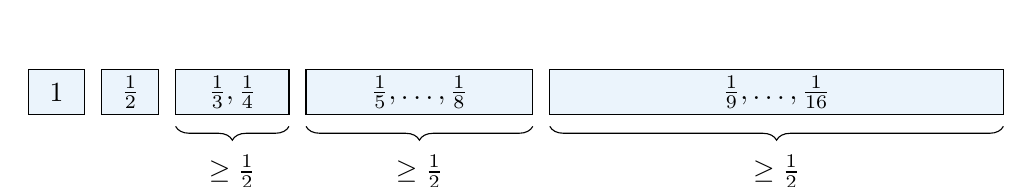
\begin{tikzpicture}[x=0.72cm,y=0.58cm,>=Latex]
  \foreach \j/\x/\w in {0/0/1,1/1.3/1,2/2.6/2,3/4.9/4,4/9.2/8}{
    \draw[fill=softblue] (\x,0) rectangle ++(\w,1);
  }
  \node at (0.5,0.5) {$1$};
  \node at (1.8,0.5) {$\frac12$};
  \node at (3.6,0.5) {$\frac13,\frac14$};
  \node at (6.9,0.5) {$\frac15,\ldots,\frac18$};
  \node at (13.2,0.5) {$\frac19,\ldots,\frac1{16}$};
  \draw[decorate,decoration={brace,amplitude=5pt,mirror}]
    (2.6,-0.25)--(4.6,-0.25) node[midway,below=7pt] {$\geq\frac12$};
  \draw[decorate,decoration={brace,amplitude=5pt,mirror}]
    (4.9,-0.25)--(8.9,-0.25) node[midway,below=7pt] {$\geq\frac12$};
  \draw[decorate,decoration={brace,amplitude=5pt,mirror}]
    (9.2,-0.25)--(17.2,-0.25) node[midway,below=7pt] {$\geq\frac12$};
\end{tikzpicture}

\small Figure 3. Infinitely many blocks each contribute at least \(1/2\), so the harmonic sums grow forever.
\end{center}

\subsection{Finish the sharpness proof}

For our test sequences, the denominator is \(H_N\) by (13). The proved inequality gives \(Q_N/H_N<4\), while (18) gives
\[
  \frac{Q_N}{H_N}>4-\frac{14}{H_N}.
\]
Since \(H_N\to\infty\),
\[
  \boxed{\displaystyle
  \lim_{N\to\infty}\frac{Q_N}{H_N}=4.}
  \tag{20}
\]
Now let \(C<4\). Choose \(N\) so large that
\[
  \frac{14}{H_N}<4-C.
\]
Then
\[
  \frac{Q_N}{H_N}>C,
\]
which means
\[
  Q_N>C\norm{c^{(N)}}_2^2.
\]
So an inequality with the smaller constant \(C\) fails. Therefore \(4\) cannot be replaced by any smaller universal constant.

\begin{ideaBox}[The important distinction]
The constant \(4\) is approached but not attained by nonzero square-summable sequences. The borderline shape \(1/\sqrt n\) would produce equality-like behavior, but
\[
  \sum_{n=1}^{\infty}\left(\frac1{\sqrt n}\right)^2
  =\sum_{n=1}^{\infty}\frac1n=\infty,
\]
so it is not an \(\ell^2\) sequence. Its finite truncations get closer and closer to the sharp constant.
\end{ideaBox}

\subsection{A numerical look}

The approach to \(4\) is slow because \(H_N\) grows only logarithmically. Here are some values of \(Q_N/H_N\):
\[
\begin{array}{rccccc}
\toprule
N&10&100&1{,}000&10{,}000&1{,}000{,}000\\
\midrule
Q_N/H_N&1.978&2.623&2.993&3.217&3.464\\
\bottomrule
\end{array}
\]
The table is not the proof; equation (20) is the proof. The table simply illustrates the slow convergence.

\section{A compact homework-ready proof}

\begin{solutionBox}[Main inequality]
Let
\[
  K_{mn}=\frac1{\max\{m,n\}},
  \qquad w_n=n^{-1/2}.
\]
For every \(m\geq1\),
\[
\begin{aligned}
 \sum_{n=1}^{\infty}K_{mn}w_n
 &=\frac1m\sum_{n=1}^{m}n^{-1/2}
   +\sum_{n=m+1}^{\infty}n^{-3/2}\\
 &<\frac1m(2\sqrt m)+\frac2{\sqrt m}
 =4w_m.
\end{aligned}
\]
Therefore, by Cauchy--Schwarz,
\[
\begin{aligned}
 \sum_{m,n\geq1}K_{mn}|a_m||b_n|
 &\leq
 \left(\sum_{m,n\geq1}K_{mn}a_m^2\frac{w_n}{w_m}\right)^{1/2}
 \left(\sum_{m,n\geq1}K_{mn}b_n^2\frac{w_m}{w_n}\right)^{1/2}\\
 &<\left(4\sum_m a_m^2\right)^{1/2}
    \left(4\sum_n b_n^2\right)^{1/2}\\
 &=4\norm a_2\norm b_2.
\end{aligned}
\]
This proves the stronger absolute-value inequality.
\end{solutionBox}

\begin{solutionBox}[Sharpness]
Take \(a_n=b_n=n^{-1/2}\) for \(n\leq N\), and \(a_n=b_n=0\) for \(n>N\). Then \(\norm a_2\norm b_2=H_N\), and
\[
\begin{aligned}
 Q_N
 &=2\sum_{m=1}^{N}m^{-3/2}\sum_{n=1}^{m}n^{-1/2}
   -\sum_{m=1}^{N}m^{-2}\\
 &>4H_N-14.
\end{aligned}
\]
Since \(H_N\to\infty\),
\[
  \frac{Q_N}{\norm a_2\norm b_2}
  =\frac{Q_N}{H_N}\longrightarrow4.
\]
Thus every constant \(C<4\) fails for all sufficiently large \(N\), so \(4\) is sharp.
\end{solutionBox}

\section{Common questions and mistakes}

\begin{warningBox}[Mistake 1: forgetting the two regions]
The formula is not \(1/m\) everywhere and not \(1/n\) everywhere. Always split at \(n=m\):
\[
 \frac1{\max\{m,n\}}=
 \begin{cases}1/m,&n\leq m,\\1/n,&n>m.\end{cases}
\]
\end{warningBox}

\begin{warningBox}[Mistake 2: applying Cauchy--Schwarz without a weight]
The proof depends on inserting
\[
  \sqrt{w_n/w_m}\sqrt{w_m/w_n}=1.
\]
Without this balancing factor, the kernel does not have a finite square sum over the whole grid.
\end{warningBox}

\begin{warningBox}[Mistake 3: saying ``sharp'' means equality occurs]
A sharp constant need not be attained. Here, nonzero \(\ell^2\) sequences satisfy a strict inequality, but truncations of \(1/\sqrt n\) make the ratio tend to \(4\).
\end{warningBox}

\begin{warningBox}[Mistake 4: forgetting to subtract the diagonal]
When a symmetric square is written as twice one triangle, the diagonal is counted twice. In the sharpness calculation, subtract \(\sum_{m=1}^{N}1/m^2\) once.
\end{warningBox}

\section{Quick self-check}

\begin{enumerate}
  \item Write the \(3\times3\) matrix \((1/\max\{m,n\})\).
  \item Why does \(\sum_{n=1}^{m}n^{-1/2}<2\sqrt m\) telescope?
  \item For a fixed \(m\), what are the two pieces of \(R_m\)?
  \item Why is the test sequence \(1/\sqrt n\) cut off after \(N\) terms?
  \item Explain in one sentence why (20) rules out every constant smaller than \(4\).
\end{enumerate}

\begin{definitionBox}[Answers]
\begin{enumerate}
  \item
  \(
  \begin{pmatrix}
  1&1/2&1/3\\
  1/2&1/2&1/3\\
  1/3&1/3&1/3
  \end{pmatrix}.
  \)
  \item Compare \(1/\sqrt n\) with \(2(\sqrt n-\sqrt{n-1})\); adjacent square-root terms cancel when summed.
  \item
  \(
  m^{-1}\sum_{n\leq m}n^{-1/2}
  \)
  and
  \(
  \sum_{n>m}n^{-3/2}.
  \)
  \item The full sequence is not square-summable because its squared terms form the divergent harmonic series.
  \item Ratios can be made arbitrarily close to \(4\), so any fixed \(C<4\) is eventually exceeded.
\end{enumerate}
\end{definitionBox}

\newpage
\section{Final map of the proof}

\begin{center}
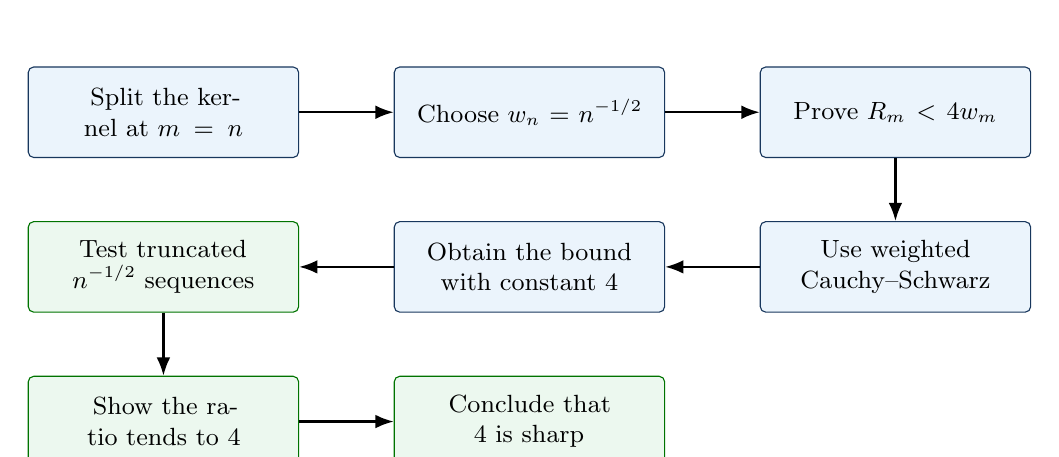
\begin{tikzpicture}[node distance=0.8cm and 1.2cm,>=Latex]
\tikzset{
  flowstep/.style={draw=navy,rounded corners=2pt,fill=softblue,
               text width=3.2cm,minimum height=1.15cm,align=center,font=\small},
  sharp/.style={draw=green!45!black,rounded corners=2pt,fill=softgreen,
                text width=3.2cm,minimum height=1.15cm,align=center,font=\small}
}
\node[flowstep] (split) {Split the kernel at $m=n$};
\node[flowstep,right=of split] (weight) {Choose $w_n=n^{-1/2}$};
\node[flowstep,right=of weight] (row) {Prove $R_m<4w_m$};
\node[flowstep,below=of row] (cs) {Use weighted Cauchy--Schwarz};
\node[flowstep,left=of cs] (bound) {Obtain the bound with constant $4$};
\node[sharp,left=of bound] (test) {Test truncated $n^{-1/2}$ sequences};
\node[sharp,below=of test] (ratio) {Show the ratio tends to $4$};
\node[sharp,right=of ratio] (done) {Conclude that $4$ is sharp};
\draw[->,thick] (split)--(weight);
\draw[->,thick] (weight)--(row);
\draw[->,thick] (row)--(cs);
\draw[->,thick] (cs)--(bound);
\draw[->,thick] (bound)--(test);
\draw[->,thick] (test)--(ratio);
\draw[->,thick] (ratio)--(done);
\end{tikzpicture}
\end{center}

\begin{ideaBox}[The whole argument in one sentence]
The square-root weight makes each row of the max-kernel cost less than \(4\), weighted Cauchy--Schwarz turns that row estimate into the desired inequality, and truncated copies of the same square-root weight show that the number \(4\) cannot be improved.
\end{ideaBox}

\end{document}
